\documentclass[12pt]{article}

\pagestyle{empty}
\setlength{\topmargin}{0in}
\setlength{\headheight}{0in}
\setlength{\topsep}{0in}
\setlength{\textheight}{9in}
\setlength{\oddsidemargin}{0in}
\setlength{\evensidemargin}{0in}
\setlength{\textwidth}{6.5in}

\usepackage{palatino,graphics,amsmath}

\newcommand{\ds}{\displaystyle}
\newcommand{\vs}[1]{\vspace{#1in}}
\renewcommand{\vss}[1]{\vspace*{#1in}}
\newcommand{\bvec}{{\mathbf b}}
\newcommand{\cvec}{{\mathbf c}}
\newcommand{\dvec}{{\mathbf d}}
\newcommand{\evec}{{\mathbf e}}
\newcommand{\fvec}{{\mathbf f}}
\newcommand{\qvec}{{\mathbf q}}
\newcommand{\uvec}{{\mathbf u}}
\newcommand{\vvec}{{\mathbf v}}
\newcommand{\wvec}{{\mathbf w}}
\newcommand{\xvec}{{\mathbf x}}
\newcommand{\yvec}{{\mathbf y}}
\newcommand{\zvec}{{\mathbf y}}
\newcommand{\zerovec}{{\mathbf 0}}
\newcommand{\real}{{\mathbb R}}
\newcommand{\twovec}[2]{\left[\begin{array}{r}#1 \\ #2
    \end{array}\right]}
\newcommand{\ctwovec}[2]{\left[\begin{array}{c}#1 \\ #2
   \end{array}\right]}
\newcommand{\threevec}[3]{\left[\begin{array}{r}#1 \\ #2 \\ #3
  \end{array}\right]}
\newcommand{\cthreevec}[3]{\left[\begin{array}{c}#1 \\ #2 \\ #3
    \end{array}\right]}
\newcommand{\fourvec}[4]{\left[\begin{array}{r}#1 \\ #2 \\ #3 \\ #4
    \end{array}\right]}
\newcommand{\cfourvec}[4]{\left[\begin{array}{c}#1 \\ #2 \\ #3 \\ #4
    \end{array}\right]}
\newcommand{\mattwo}[4]{\left[\begin{array}{rr}#1 \amp #2 \\ #3 \amp #4 \\ \end{array}\right]}

\begin{document}

\noindent
{\bf Mathematics 227} \\ 
{\bf Vectors}

\bigskip
Suppose that
$$
\vvec = \twovec{3}{1}, \wvec=\twovec{-1}{2}.
$$

\begin{enumerate}
\item Find expressions for the vectors
  $$
  \begin{array}{cccc}
    \vvec, & 2\vvec, & -\vvec, & -2\vvec, \\
    \wvec, & 2\wvec, & -\wvec, & -2\wvec. \\
  \end{array}
  $$
  and sketch them below.

  \bigskip
  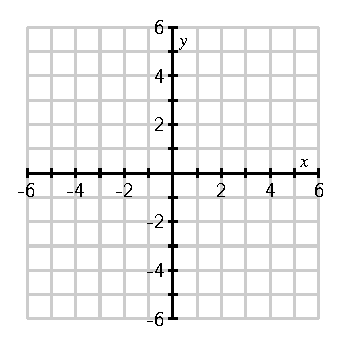
\includegraphics{empty-6.eps}

\item What geometric effect does scalar multiplication have on a
  vector?  Also, describe the effect that multiplying by a negative
  scalar has.

  \vs{1}

\item Sketch the vectors $\vvec$, $\wvec$, and $\vvec+\wvec$.
  
  \bigskip
  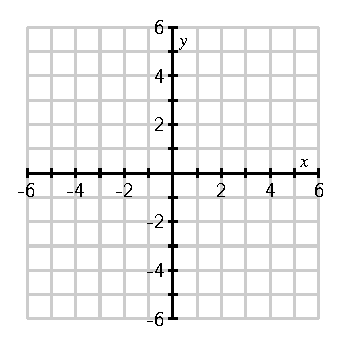
\includegraphics{empty-6.eps}

\item Consider vectors that have the form $\vvec+a\wvec$ where $a$ is
  any scalar. Sketch a few of these vectors when, say, $a=−2,−1,0,1,$ and
  2. Give a geometric description of this set of vectors.  

  \bigskip
  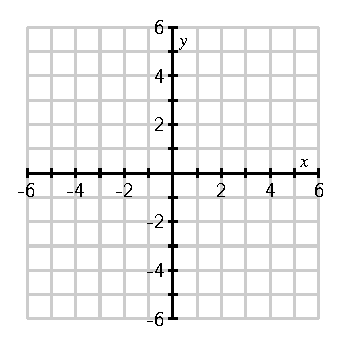
\includegraphics{empty-6.eps}

\item If $a$ and $b$ are two scalars, then the vector
  $$
  a\vvec+b\wvec
  $$
  is called a {\em linear combination} of the vectors $\vvec$ and
  $\wvec$.  Find the vector that is the linear combination when $a=-2$
  and $b=1$.

  \vs{1.5}
\item Can the vector $\twovec{-31}{37}$ be represented as a linear
  combination of $\vvec$ and $\wvec$?  In other words, can you find
  scalars $a$ and $b$ such that $a\vvec + b\wvec = \twovec{-31}{37}$. 

\end{enumerate}


\end{document}
